\part{L'édition numérique des corpus de Louis II, d'Anne Dauphine et de Charles I\up{er} et d'Agnès de Bourgogne}


\newpage

	\chapter{Présentation du corpus}

\vspace*{\stretch{1.3}} 
\par Le corpus dénombre huit cent vingt-trois actes, avec presque autant d'actes pour chaque couple de prince. Quatre cent douze actes sont recensés pour Louis II (333) et Anne Dauphine (79) et quatre cent six actes pour Charles I\textsuperscript{er} (379) et Agnès de Bourgogne (32). L'étude de ce corpus est permise par la conservation des différents actes étudiés. Lorsqu'on y regarde de plus près, on est vite confronté  à la dispersion de la documentation. Aucune série documentaire ne se rapporte à la chancellerie ni ne contient l'enregistrement des actes des ducs de Bourbon par cette dernière\footnote{\cite{matteoniEcriturePouvoirPrincier2011}.}.
\vspace*{\stretch{0.7}} 
\newpage 

\section{Dispersion des actes}
\label{I.1.1}

\par Les actes des Bourbons sont conservés depuis le \textsc{XII}\up{e} siècle\footnote{\cite{huillard-brehollesTitresMaisonDucale1867}.}. Sous la première maison de Bourbon, les seigneurs de Bourbon-Dampierre, les pièces originales sont déposées dans des coffres ou des layettes et les lettres sont petit à petit transcrites dans des cartulaires. L'accroissement de la production documentaire donne lieu à la réalisation d'inventaires dès le \textsc{XIV}\up{e} siècle. Après la création de la chambre des comptes de Moulins, en 1374, le duc Louis II  ordonne que tous les actes, terriers, lettres et écritures touchant au domaine (nominations, lettres de dons et de grâce, ordonnances) y soient remis\footnote{\cite{huillard-brehollesTitresMaisonDucale1867}.}. La chambre des comptes se sédentarise à Moulins et fonctionne avec une régularité croissante. Le \og Trésor des chartes\fg \space du Bourbonnais s'agrandit et est complété par les inventaires des actes conservés dans les territoires nouvellement acquis. En effet, Louis II maintient les Chambres des comptes du comté de Forez à Montbrison et de la seigneurie de Beaujolais à Villefranche. En 1527, cinq ans après de la fuite du dernier duc de Bourbon, le connétable Charles III~(1505~-~1523), François I\up{er}~(1515~-~1547) confisque tous les biens féodaux des Bourbons tenus en apanage\footnote{\cite{huillard-brehollesTitresMaisonDucale1867}.}. L'administration des domaines revient alors à la mère du roi, Louise de Savoie~(1476~-~1531), petite fille du duc de Bourbon Charles I\up{er}, qui en revendique alors la possession. À sa mort, cet héritage contesté retourne à la couronne. Les chambres des comptes du duché de Bourbon sont supprimées, leur juridiction est transférée à la chambre des comptes de Paris et le Trésor des chartes du Bourbonnais y est rapatrié après la réalisation d'un inventaire par Jacques Luillier\footnote{\cite{huillard-brehollesTitresMaisonDucale1867}.}. Au début du \textsc{XVIII}\up{e} siècle, pour éviter les pertes, les liasses sont reliées et converties en volumes et les sceaux sont coupés. Le tout est réuni dans le dépôt de la chambre d'Anjou. La série de titres et de registre qui était restée à Moulins est détruite sous le Directoire comme entaché de féodalité, celle de Villefranche subit de nombreuses pertes et les archives du Forez à Montbrison sont transférées à Lyon au bureau des trésoriers de France. L'inventaire des \textit{Titres des Bourbons}\footnote{\cite{huillard-brehollesTitresMaisonDucale1867}.}, édité par les archivistes Alphonse Huillard-Bréholles et Albert Lecoy de la Marche au \textsc{XIX}\up{e} siècle, dresse, de manière chronologique, la liste des actes des trois chambres des comptes du duché qui sont conservés dans la série P des Archives nationales, dans les fonds des anciennes Chambre des comptes du duché de Bourbon (P 1355 à P 1402)\footnote{Archives nationales, Série P, Chambre des comptes et comptabilité, en ligne : \url{http://www.archivesnationales.culture.gouv.fr/chan/chan/fonds/EGF/SA/SAPDF/Egfn-p.pdf}.}. La majorité des actes du corpus (318) provient de cette série P, mais quelques actes ont également été identifiés dans les séries J~(43) et K~(7)\footnote{Série J, Trésor des Chartes - Série K, Monuments historiques.}. 

\par Une autre partie importante du corpus est issue des services d'archives départementales (221). La localisation de ces institutions de conservation révèle la géographie du duché de Bourbon. La majorité des actes identifiés aux Archives départementales provient du service de la Loire (150). Le territoire de ce département correspond à celui de l’ancien comté de Forez, qui est rattaché à la principauté par héritage lors du mariage, en 1371, entre Louis II et Anne Dauphine. D'autres actes sont conservés dans les services de l'Allier, sur le territoire du duché de Bourbonnais, du Puy-de-Dôme, sur le territoire du duché d'Auvergne et du Cantal, dont une partie était autrefois rattaché au duché d'Auvergne. Les actes conservés dans les services d'archives municipales nous éclairent également sur la géographie de la production documentaire des ducs de Bourbon. Des actes ont été identifiés dans les services d'archives de Moulins, capitale du duché. Louis II y fait construire un château en 1375 et s'y installe définitivement. Ses successeurs font de même et la ville devient alors le siège de la cour ducale et un centre culturel important\footnote{« Les ducs de Bourbon, le roi et le royaume de France à la fin du Moyen Âge », in : \cite{matteoniBourbonsLeurBibliotheque2022}}. D'autres actes ont été retrouvés aux Archives municipales de Riom, la capitale du duché d'Auvergne, et de Montluçon, une autre ville d'envergure. Ils sont, pour la grande majorité, relatifs à l'administration de la principauté bourbonnaise. 
\newline 

\par La localisation des institutions de conservation témoigne également des relations entretenues par les Bourbons avec les autres princes. Des actes proviennent des services d'archives départementales de la Côte-d'Or (24), et du Nord (ancien duché de Flandres) pour le corpus de Charles I\up{er}, et témoignent des alliances et accords passés avec les ducs de Bourgogne. D'abord, son mariage, en 1425, avec Agnès, la fille du duc Jean Sans Peur\footnote{AN, P 1370\up{2}, c. 1919. (4 février 1425).}, puis des traités et des abstinences de guerre conclues avec Philippe le Bon\footnote{AD Côte-d’Or, B 11918, c. 118. (4 décembre 1434).}. En moindres proportions, des actes ont été recensés dans les services d'archives départementales de la Loire-Atlantique et du Tarn. Ils témoignent des liens entre les différents princes et des différentes alliances et trêves conclues pendant la guerre de Cent Ans\footnote{AD Nord, B 304, c. 15.660 (7 septembre 1435) — AD Loire-Atlantique, E 121-1, c. 42 (4 avril 1441).}. Le reste des actes du corpus provient de la Bibliothèque nationale de France (172), notamment de la collection Gaignière\footnote{BnF, ms. fr. 22388 et 22390.}, ou de collections d'érudits des \textsc{XVII}\up{e} - \textsc{XVIII}\up{e} siècles (La Mure, Hozier, Tripperet). 

\par Le corpus étudié est donc dispersé géographiquement, institutionnellement et chronologiquement dans la mesure où il se déploie sur plus d'un siècle. 

\section{Répartition chronologique des actes}
\label{I.1.2}

\par Le corpus étudié couvre la période allant de 1357 à 1475. Nous pouvons établir une première période allant de 1357 à 1410 pour Louis II et jusqu'à 1417 pour Anne Dauphine. Puis, une seconde période de 1421 à 1456 pour Charles I\textsuperscript{er} et jusqu'à 1475 pour Agnès de Bourgogne. Les veuves des deux ducs leur survivent et continuent à produire des actes en raison des circonstances politiques. Anne Dauphine continue à émettre des actes pour le comté de Forez, dont elle est l'héritière, et au début de la captivité de Jean I\up{er}.
\newline 

\par À partir du graphique ci-après, nous pouvons établir une moyenne d'environ dix actes par an pour notre corpus. Le nombre d'actes est en deçà au début du principat de Louis II. En revanche, on observe une augmentation des écrits à partir des années 1380, qui fait suite à ses réformes administratives. Ensuite, le nombre d'actes recensés est plutôt stable jusqu'à sa mort. 

\begin{figure}[ht]
\centering
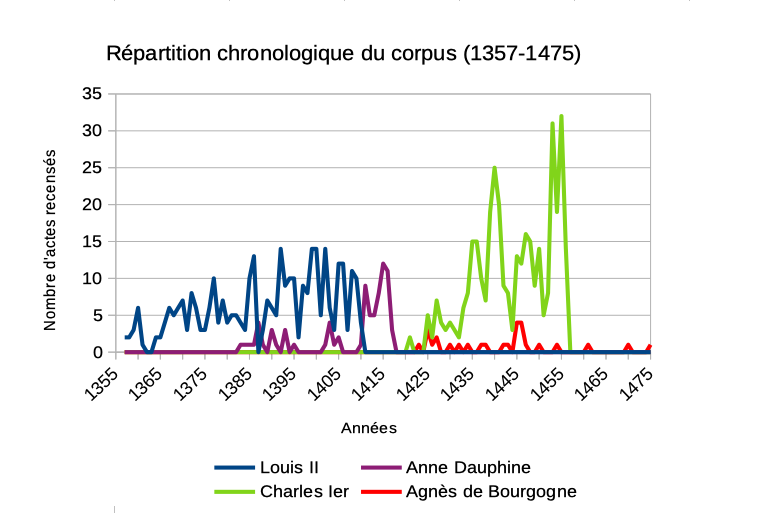
\includegraphics[scale=0.6]{front/images/repartition_chronologique_corpus.png}\caption{Répartition chronologique des actes du corpus.} \label{fig:chrono_actes}
\end{figure}
\newpage 

\par La diminution du nombre d'actes entre le principat de Louis II et celui de Charles~I\textsuperscript{er} s'explique par le fait que Charles I\up{er} n'est pas le successeur direct de Louis II d'une part. D'autre part, les actes du duc Jean~I\textsuperscript{er} et de son épouse Marie de Berry ne sont pour l'instant pas traités par le projet Actes princiers. Néanmoins, des actes sont quand même le fait de la duchesse Anne Dauphine, pour laquelle on observe une nette augmentation à la mort de son époux, et de Charles de Bourbon, qui commence à administrer le duché pendant la captivité de son père. Le nombre d'actes recensés pendant le principat de Charles I\textsuperscript{er}, à partir de 1434, est caractérisé par une augmentation par rapport à la période de Louis II, ce qui peut faire penser à une émission de plus d'actes sur une plus courte période. Cette augmentation peut s'expliquer par la consolidation d'une administration déjà stable, mais surtout par le biais documentaire qu'induit le corpus. Nous ne pouvons en effet pas chiffrer la part de la production totale de la chancellerie bourbonnaise qui nous est parvenue par rapport à celle qui a été perdue. L'un des pics de production peut être documenté plus assurément. Il s'agit de l'augmentation au début des années 1440, pendant la Praguerie\footnote{\cite{generoChanceliersSecretairesChancellerie2021}.}, avec de nombreuses nominations de capitaines-châtelain et de capitaines de guerre\footnote{BnF, ms. fr. 22299, folio 9 (20 juillet 1440) — BnF, ms. fr. 22299, folio 9 (30 juillet 1440).}. Cependant, le second pic en 1455, peu avant la mort du duc, avec de nombreuses nominations et fondations pieuses afférentes au duché\footnote{\cite{matteoniServirPrinceOfficiers1994}.}, ne peut réellement être explicité. Il est certainement plutôt dû à un effet de source qu'à un regain administratif à la fin de la vie de Charles I\textsuperscript{er}. En effet, nous conservons un registre d'enregistrement d'actes de la Chambre des comptes du comté de Forez, à Montbrison, qui contient des copies de lettres de nomination d'officiers des années 1450 aux années 1470\footnote{AD Loire, B 1844.}.
\newline 

\par L'émission des actes est plutôt 
constante malgré quelques variations dues au contexte politique du duché pour la période étudiée. Néanmoins, il ne faut pas perdre de vue que ce graphique omet les actes qui ont été perdus, ou qui n'ont pas encore été retrouvés, et comptabilise le corpus étudié, soit les actes qui ont été identifiés. Ces derniers représentent une masse conséquente aux natures et aux typologies variées. 
\newpage 

\section{Typologie des actes}
\label{I.1.3}

\par L'étude du corpus révèle les différentes typologies documentaires. Parmi les actes à forte valeur juridique, on trouve des chartes, dont la valeur est perpétuelle, et des lettres patentes qui accordent une faveur au destinataire. Dans une moindre mesure, on trouve aussi des lettres closes, fermées d'un sceau, et des lettres missives, ces dernières ayant plus un caractère politique puisqu'elles sont destinées à une correspondance officielle. Des écrits sont dédiés à l'administration du duché, en témoignent les nombreux mandements, des ordres du prince, concernant la gestion du domaine et des quittances qui attestent du remboursement de sommes dues. Certains actes sont plus singuliers, comme les accords passés avec d'autres princes, dans la mesure où ils comportent les titulatures des deux individus\footnote{AN, P 1357\textsuperscript{2}, n° 428 (avril 1372).}, et les différentes versions des testaments des ducs de Bourbon\footnote{AN, P 1370\textsuperscript{1}, c. 18791 (12 décembre 1428) — AN, P 1370\textsuperscript{1}, c. 1880 (4 décembre 1456).}. Pour chaque duc et duchesse, on recense ces différents types d'actes. Les corpus sont diversifiés, hormis celui d'Agnès de Bourgogne (essentiellement des quittances et des missives). 
\newline 

\begin{figure}[ht]
\centering
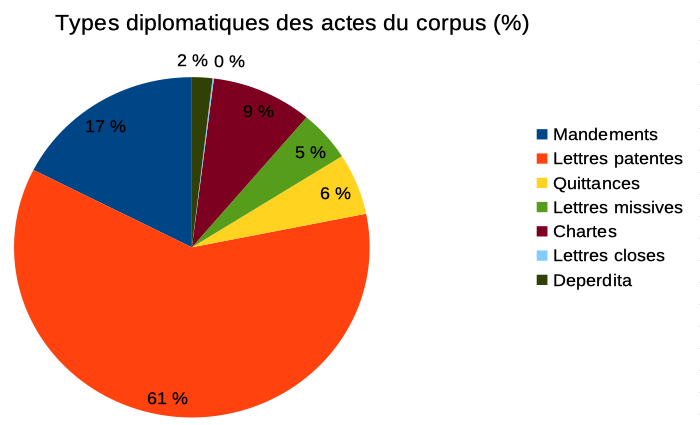
\includegraphics[scale=0.6]{front/images/typologie_documentaire.png}
\caption{Typologie des actes étudiés.}
\label{fig:typo_actes}
\end{figure}
\newpage 

\par  Comme le montre le graphique ci-avant, les lettres patentes sont majoritaires. Ce sont des actes à caractère juridique exprimant la volonté du duc. Ces lettres sont généralement destinées à des particuliers et beaucoup d'entre elles entérinent des nominations d'officiers, des souffrances d'hommages ou encore des donations ...\footnote{AN, P 1374\textsuperscript{2}, n° 2420 (19 février 1403) — AD Loire, B 1844, folio n°4 recto (21 mai 1453).}. Le deuxième type d'acte le plus représenté est le mandement. Ils concernent en majorité Louis II, et ce tout au long de la période\footnote{AN, P 1376\textsuperscript{2}, n° 2749 (27 février 1457) — AN, P 1389\textsuperscript{3}, n° 370 (30 juin 1410).}, et dans une moindre mesure Charles I\textsuperscript{er}\footnote{BnF, ms. fr. 20389, c. 78 (20 juin 1444).}. Ces actes ont trait à l'administration instante du duché : paiement de taxes, impositions extraordinaires, saisies, réparations diverses et fortifications, enquêtes, requêtes ...\footnote{AN, K 48, n° 6 (5 mai 1360) — AM Montluçon, AA 8 (1) (20 novembre 1360) — AM Montluçon, AA 2 (1) (1368) — AM Montluçon, n° 240, boîte 3 (7 novembre 1373) — AN, P 1376\up{2}, n° 2716 (25 août 1376) — AN, P 1379\up{2}, c. 3136/16 (18 août 1437) — AN, P 13911, c. 562 (23 mai 1447).}. Viennent ensuite les quittances et les chartes. Cette production a trait principalement aux finances (aides et paiements), à l'administration, ces deux aspects étant intimement liés, et enfin aux relations entretenues avec le roi et les autres princes. Les documents relatifs à la gestion du domaine font preuve d’une grande variété : aides, documents relatifs à l’organisation des marchés et des foires dans les localités relevant de la juridiction\footnote{AN, P 1376\textsuperscript{2}, n° 2752 (10 septembre 1366).}, et dans une moindre mesure des fondations pieuses\footnote{AN, P 1355\textsuperscript{1}, n° 46 (18 août 1392).}. Quelques mentions de trêves, d’organisation d'États ont également été relevées. Une partie de la production documentaire du duché est liée au contexte de guerre de Cent Ans : des actes mentionnent des autorisations de fortification\footnote{AD de la Loire, B 1952 (1\textsuperscript{er} mai 1435).}, des nominations de capitaines\footnote{BnF, ms. fr. 22299, folio 7 (24 octobre 1439).} et des garnisons. Les documents afférant aux relations du duc avec les grands du royaume enregistrent des alliances\footnote{AN, P 1372\textsuperscript{2}, c. 2113, (4 août 1427).}, des trêves\footnote{AD de la Côte-d’Or, B 11918, c. 117 (24 octobre 1433).}, des promesses\footnote{AD de la Côte-d’Or, B 11904, c. 67 (6 février 1436).}, mais aussi des ambassades\footnote{AN, P 1360\textsuperscript{2}, c. 881 (28 mai 1431).}, des ratifications de paix\footnote{AD du Nord, B 304, c. 15.660 (1\textsuperscript{er} octobre 1435).} ou des tractations relatives aux otages\footnote{Mention : Aubret L., Mémoires pour servir à l’histoire de Dombes, II, Guigue M.-C. (éd.), Trévoux, 1868, p. 617. Indication de provenance : \og Titres de Trévoux \fg.}. L’autre partie consiste en des ratifications de conventions de mariage\footnote{AN, P 1370\textsuperscript{2}, c. 1919 (4 février 1425).} et en paiements de dots\footnote{AD de la Côte-d’Or, B 299, pièce scellée 338 (8 décembre 1425).}. 
\newpage 

\par Malgré quelques tensions avec le roi lors de la Praguerie, Charles I\textsuperscript{er} mène une politique d’alliances par les mariages de ses enfants (Anjou, France, Bourgogne)\footnote{AN, P 1370\textsuperscript{2}, c. 1915 (14 février 1437).} et affirme sa place au rang de prince via l’écrit et la représentation. Cette production, riche et abondante, participe à la consolidation administrative qui caractérise la période. En témoigne la création des offices de gouverneur général des finances (1437) et de contrôleur général (1445)\footnote{\cite{matteoniServirPrinceOfficiers1994}}. En fin de vie, on observe une augmentation des fondations pieuses ainsi que la présence de lettres personnelles adressées à des membres de la famille, c'est notamment le cas pour le corpus d'Agnès de Bourgogne\footnote{AN, K 188, c. 304 (18 novembre 1470) — BnF, ms. fr. 15538, folio 138 (11 novembre, après 1473).}. Quelques \textit{deperdita} ont été recensés, des actes perdus ou détruits dont l'existence est attestée par une mention. Néanmoins, ils ne sont pas très représentatifs de l'ensemble du corpus puisqu'ils font en grande majorité partie du corpus de Charles I\textsuperscript{er}. Les archives des ducs de Bourbon sont progressivement versées à la chambre des comptes de Paris lors du rattachement du duché à la couronne. Une partie de ces actes a disparu dans l'incendie de la chambre des comptes de 1737, et nous est connu par des inventaires\footnote{\cite{nortierSortArchivesDispersees1965}.}. La collection de l'historiographe et collectionneur François Roger de Gaignières, donne les analyses de nombreux actes de notre corpus\footnote{BnF, ms. fr. 22388 et 22390.}. 
\newline 

\par Les actes recensés révèlent des typologies variées et offrent, malgré les pertes documentaires, un riche extrait de ce à quoi pouvait ressembler la production documentaire pour la période étudiée. Nonobstant la diversité typologique qui les caractérise, les actes émis par les ducs de Bourbon ne sont pas dépourvus de ressemblance avec les actes royaux.
\newpage 

\section[Pratiques d'\textit{imitatio regis}]{L'\textit{Imitatio regis} au c\oe{}ur des pratiques documentaires des princes de Bourbon}
\label{I.1.4}

\par Les princes du royaume de France adoptent le modèle royal en imitant les usages diplomatiques de la chancellerie royale. Même si ce modèle ne s’impose pas unanimement pour des raisons politiques (Bretagne, Bourgogne\footnote{Originalité qui va disparaître lorsque les Valois mettront la main sur le duché,  \cite{courtelChancellerieActesEudes1977}.}) ou à cause de l'usage de pratiques locales, la majorité des actes émis par les chancelleries ducales présentent de nombreuses similitudes avec les actes royaux. Olivier Canteaut relève que \og l'imitation ou le rejet des modèles sont autant d'instruments qui permettent aux autorités d’affirmer leur domination sur leurs sujets et leur identité politique face à leurs correspondants étrangers \fg\footnote{\og Introduction\fg, in : \cite{canteautDiscretLangagePouvoir2019}.}. En tant que branche cadette de la famille royale depuis le \textsc{XIII}\textsuperscript{e} siècle (descendants de Saint-Louis~(1226~-~1270)), les Bourbons bénéficient de l'office héréditaire de grand chambrier de France\footnote{Grand chambrier : grand officier de la couronne chargé de l'intendance de la chambre du roi et de la garde du trésor royal. Définition CNRTL : \url{https://www.cnrtl.fr/definition/chambrier}.} et d'une proximité particulière avec les rois de France\footnote{\og Les ducs de Bourbon, le roi et le royaume de France à la fin du Moyen Âge \fg, in : \cite{matteoniBourbonsLeurBibliotheque2022}.}. La participation de Louis II au gouvernement du royaume dès la minorité de son neveu Charles VI, ainsi que ses nombreux déplacements accompagnés de sa chancellerie, ont favorisé la circulation des conseils, des savoir-faire et des modèles\footnote{\cite{matteoniEcriturePouvoirPrincier2011}.}. La chancellerie est l’organe producteur de l'écrit princier, mais aussi de l'image et du discours du prince\footnote{\cite{generoChancellerieCharlesIer2018}.}. Celle des ducs de Bourbon, localisée à Moulins, est semblable en de nombreux points à la chancellerie royale dans son organisation, mais aussi dans la production des écrits. De plus, les \textsc{XIV}\textsuperscript{e} - \textsc{XV}\textsuperscript{e} siècles voient l'émergence et la réapparition de la figure du chancelier, l'officier chargé de l'écrit et de la garde du sceau. Il est en ce sens le responsable de la mise par écrit de la volonté politique du prince par la vérification des actes et leur signature une fois ceux-ci conformes. Olivier Guyotjeannin indique que \og se doter d’un chancelier, homme de culture juridique, rompu aux jeux du pouvoir, attiré vers la justice en ce qu’elle est le condensé du gouvernement des hommes, apparaît ainsi bien souvent comme le premier acte de l’identité diplomatique princière \fg\footnote{Conclusion par Olivier Guyotjeannin \cite{matteoniEcriturePouvoirPrincier2011}.}. Les officiers en charge de l'écrit princier sont les secrétaires, des professionnels de l'écrit public. Après délibérations du conseil ducal, et en fonction des directives de ce dernier, les secrétaires rédigent des minutes, des premières rédactions d'un acte. Les minutes sont ensuite grossoyées au propre par des clercs. La production documentaire relative à l'administration du duché de Bourbon est exécutée par des hommes qualifiés qui irriguent le milieu politico-administratif et financier bourbonnais. Ce sont majoritairement des érudits laïcs (licenciés en droit ou bacheliers en décret), dont les qualités mentionnées dans les lettres de nomination font référence à la science, à la probité, à la diligence et à la vertu\footnote{\cite{matteoniEcriturePouvoirPrincier2011}.}.  On dénombre quinze officiers chargés de l'écrit ducal sous Louis II\footnote{\cite{matteoniEcriturePouvoirPrincier2011}.} et trois chanceliers et vingt-huit secrétaires entre 1425 et 1456 (quatorze pour Charles I\textsuperscript{er} et neuf pour Agnès de Bourgogne)\footnote{\cite{generoChancellerieCharlesIer2018}.}. Ils sont généralement issus de la bourgeoisie locale, sauf quelques exceptions. Parmi elles, nous pouvons citer le cas d'Etienne de Bar, talentueux secrétaire venu de Paris, auparavant secrétaire du roi\footnote{\cite{matteoniEcriturePouvoirPrincier2011}.}. Même s'il reste isolé, ce cas de figure a pu jouer dans l'adoption des pratiques d’écriture en vigueur à la chancellerie royale.
\newline 

\par Cette pratique d'\textit{imitatio regis}\footnote{Mélissa Barry, Cléo Rager, Élisabeth Schmit, Marie-Émeline Sterlin et Clémence Lescuyer, \og \og Imitatio regis \fg ? Pour une diplomatique des actes de Jean de Berry\fg, in : \cite{guyotjeanninJeanBerryEcrit2019}.} est visible dans les écrits, au sein des caractères externes des actes. La réalisation est soignée, l'écriture conforme au modèle royal, avec des abréviations canoniques et peu nombreuses. L'organisation des différentes parties du discours suit celle des actes royaux sur un format horizontal : exposé, mentions hors teneurs, signatures organisées autour d'un paraphe cadre. Des emprunts très caractéristiques ont trait à l'ornementation avec l'utilisation de fleurs de lys, motifs typiques de l’iconographie des chartes royales contemporaines des Valois\footnote{Annexe Initiales fleurdelisées. \newline AN, P 1363\up{1}, c. 1151\up{1} (18 décembre 1448) – AN, P 1368\up{2}, c. 1628 (19 février 1447).}. Ce discours dynastique et sacré est également présent sous le principat de Charles I\textsuperscript{er}\footnote{\cite{generoSceauxArmesCharles2022}.}. On remarque des anges sur le sceau ducal et un usage plus affirmé du sceau du secret à partir des années 1440. Cette \textit{imitatio} est également manifeste dans les caractères internes des actes. Le vocabulaire de l'exposé, le contenu des clauses, la forme de la datation ainsi que la notification \og a tous présens et a venir \fg \space ou \og a tous ceux qui ces presentes verront \fg \space témoignent d'une proximité importante avec la chancellerie royale. L'organisation des parties du discours et le vocabulaire suivent ceux en usage à la cour du roi de France. Néanmoins, quelques dissemblances peuvent être relevées. Les différences majeures se rapportent aux verbes usités et à la langue des actes. En Bourbonnais, la langue vernaculaire domine. Les quelques actes rédigés en latin sont généralement des actes très solennels destinés aux clercs et aux institutions religieuses. 
\newline
\par La structuration de la chancellerie sous Louis II et sa prolongation sous Charles I\textsuperscript{er} marque un approfondissement de l'\textit{imitatio regis} qui traduit l'attachement familial des Bourbons au lignage des rois de France et une volonté d'asseoir leur pouvoir par l'imitation du modèle royal. Le rôle des individus, notamment des officiers de la chancellerie, est également à souligner dans la diffusion des pratiques d’écriture pour la période étudiée. 
\newline 
\newline 
\par Le corpus rassemble des actes princiers aux typologies variées, dispersés au gré des différentes institutions de conservation et s'échelonnant sur une période de plus d'un siècle. La production recensée qui a permis de former le corpus étudié est le fruit d'un travail de longue haleine de regroupement puis d'édition des actes. 

\newpage
\thispagestyle{empty}
\mbox{}
\newpage
 
	\chapter[Éditions numériques]{Des éditions numériques à partir d'un logiciel de traitement de texte}

\vspace*{\stretch{1.3}} 
\par Les premiers projets d'édition sont impulsés par des érudits au \textsc{XIX}\textsuperscript{e} siècle, avec comme objectif principal de rassembler des corpus et d'en fournir les éléments d'analyse\footnote{\og L'évolution des pratiques éditoriales \fg, in : \cite{guyotjeanninConseilsPourEdition2009}.}. Les actes des princes laïcs sont quelque peu délaissés par ces entreprises au profit des actes pontificaux et royaux. Les perspectives qu'offre aujourd'hui le numérique permettent l'étude de corpus importants et dispersés sur un temps indéterminé, autant de possibilités que n'offre pas la publication d'un ouvrage, comprenant ainsi la reproduction, la publication et la diffusion de documents d'archives. C'est dans ce contexte que l'on voit se développer des entreprises d'édition consacrées aux actes princiers et dans lequel s'inscrivent les éditions des actes émis par les Bourbons. 
\vspace*{\stretch{0.7}} 
\newpage 

\section{Trois projets d'édition}
\label{I.2.1}

\vspace*{\stretch{0.1}} 
\par Les quatre corpus rassemblant les actes de Louis II, d'Anne Dauphine, de Charles I\up{er} et d'Agnès de Bourgogne sont stockés, au commencement du stage sur lequel ce mémoire s'appuie, dans des fichiers de traitement de texte. Ces fichiers ont été constitués à l'issue du travail de recensement des actes dans les différentes institutions citées précédemment. Il s'agit d'éditions critiques : des éditions spécifiques qui collationnent les variantes d’un texte tout en pourvoyant ce dernier d’un apparat critique\footnote{L'apparat critique désigne l'ensemble des annotations d'érudition qu'un éditeur ajoute à un texte original. \og Le destin de l'appareil critique dans l'édition scientifique numérique\fg, in : \cite{apollonEditionCritiqueEre2017}.}. 
\newline 

\par Ces éditions ont été menées par plusieurs chercheurs, sur des temporalités différentes et avec des objectifs différents : recherches personnelles, mémoire académique et travail préparatoire d'une communication scientifique. Les actes de Louis II ont été édités par Olivier Mattéoni, enseignant chercheur à l'Université Paris 1 Panthéon-Sorbonne, dans le cadre de ses recherches sur les Bourbons\footnote{\cite{matteoniEcriturePouvoirPrincier2011}}. Il a notamment soutenu une thèse de doctorat sur les officiers bourbonnais en 1994 et publié de nombreux travaux sur le duché et les ducs de Bourbon\footnote{\cite{matteoniServirPrinceOfficiers1994}.}. Les actes de Charles I\up{er} et d'Agnès de Bourgogne ont été édités par Jean-Damien Généro pour son mémoire de Master recherche soutenu à l'Université Panthéon-Sorbonne en 2018, sous la direction d'O. Mattéoni\footnote{\cite{generoChancellerieCharlesIer2018}.}. Les actes d'Anne Dauphine ont enfin été édités conjointement par O. Mattéoni et J.-D. Généro en vue de présenter une communication sur la diplomatique de la duchesse au colloque organisé en 2017 pour les cinq cents ans de sa mort\footnote{\cite{matteoniActesAnneDauphine2019}.}.O. Mattéoni a par la suite retravaillé les fichiers de Louis II et d'Anne Dauphine en systématisant l'ajout des notes critiques qui concernent les individus et les lieux. Il a aussi rédigé de succinctes biographies des individus qui apparaissent régulièrement dans les actes (les grands officiers, les grands prélats) et les a ajoutées comme note critique à chaque fois que ces individus apparaissent. Pour les lieux, il a précisé leurs localisations (toponyme actuel, canton, département). Dans la mesure où il n'est pas possible de prévoir comment les utilisateurs vont aborder le corpus sur le site internet ni quel sera soit leur point d'entrée, l'existence de notes concernant les individus et les lieux demeure essentielle. 

\par Les éditions des actes de Louis II et d'Anne Dauphine n'étaient pas destinées à être immédiatement éditées sous forme papier ou électronique, tandis que celles des actes de Charles I\up{er} et d'Agnès de Bourgogne ont été imprimées dans le cadre d'un travail universitaire. Ces finalités différentes supposent des choix de mise en forme et de mise en page différents, qui ont une influence sur les traitements postérieurs. En effet, concevoir un fichier de traitement de texte dans le but de l'imprimer implique de privilégier les aspects visuels de l’édition et sa mise en page.

\par Les actes ont été édités grâce à un logiciel de traitement de texte. Le traitement de texte qualifie les logiciels qui permettent à un utilisateur de rédiger du contenu informatisé. Ces logiciels sont multiples et utilisent différents formats (ODT, docx) plus ou moins compatibles selon les logiciels et les systèmes d'exploitation. Un format de fichier spécifie la manière dont les données sont stockées pour une application particulière \footnote{Microsoft, \og En apprendre plus sur les formats de fichiers\fg, \url{https://support.microsoft.com/fr-fr/office/en-apprendre-plus-sur-les-formats-de-fichiers-56dc3b55-7681-402e-a727-c59fa0884b30}.}. La lecture des différents formats et de leur mise en forme diffère selon les applications. J.-D. Généro a édité les actes de de Charles I\up{er} et d'Agnès de Bourgogne sur le logiciel de traitement de texte \textit{Pages} de MacOS avant de les convertir en ODT. Les actes d'Anne Dauphine ont également été édités sur un fichier ODT tandis que les actes de Louis II ont été édités sur un fichier docx. Le fichier docx est un document Microsoft Word au format Open XML et le fichier ODT est un document LibreOffice au format OpenDocument. Même si OpenDocument Format (ODF) prend en charge les fonctionnalités OpenOffice et Open XML, et que Microsoft Office prend en charge ODF, toutes les fonctionnalités ne sont pas prises en charge, ce qui peut occasionner des changements en termes de modification d’un document et des pertes de contenu.

\par Les travaux de recherche, même à leurs prémisses, sont rarement neutres, puisque les données ne le sont pas non plus, et qu'ils consistent en la reprise de données qui ont souvent déjà été traitées. Les fichiers de traitement de texte peuvent être qualifiés de \textit{legacy data}, puisqu'ils sont le résultat de traitements antérieurs opérés par les premiers chercheurs à travailler sur le corpus\footnote{Sur le concept de \textit{legacy data}, voir : \cite{reignierVersIndexationAutomatique2022}.}. Les ingénieurs du projet \og Actes princiers\fg \space ont conscience qu'ils vont devoir composer avec cela tout au long de leurs traitements et intégrer ce paramètre à leur réflexion.
\newline 

\par Ces différences de finalités et de formats posent des problèmes d'harmonisation des données lorsqu'il s'agit de regrouper les actes des ducs de Bourbon pour en proposer une édition cumulative. Malgré ces disparités dans la mise en page, les éditions comportent des similitudes, notamment dans leurs présentations que l'on peut qualifier de diplomatiques.
\newpage

\section{Des éditions diplomatiques}
\label{I.2.2}

\par Les différentes éditions suivent les normes en vigueur développées dans les \textit{Conseils pour l'édition des textes médiévaux} de l'École Nationale des Chartes\footnote{\cite{guyotjeanninConseilsPourEdition2014}. - \cite{guyotjeanninConseilsPourEdition2009}.}, inspirés des règles établies en 1984\footnote{\cite{c.i.d.NormesInternationalesPour1984}.}. Les actes médiévaux étant généralement écrits d'un seul bloc, il est d'usage de restituer cette mise en forme en éditant le contenu textuel de l'acte en un seul paragraphe. Le texte édité est accompagné d'éléments de présentation. Comme l'explique Olivier Guyotjeannin, \og une fois le texte établi et son apparat mis en forme, il reste à le munir d'un "habillage", composé des éléments de présentation qui guideront la lecture. L'éditeur cherche à concilier le respect d'éléments qui peuvent être signifiants et les commodités fournies au lecteur contemporain \fg \footnote{\og La présentation de l'édition \fg, in : \cite{guyotjeanninConseilsPourEdition2009}.}. 
\newline 

\begin{figure}[ht]
\centering
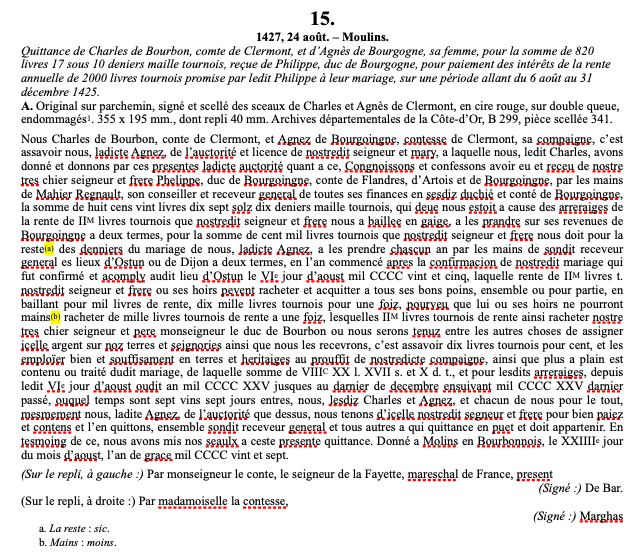
\includegraphics[scale =0.6]{front/images/edition.png}
\caption{Édition diplomatique de l'acte daté du 27 août 1427.}
\label{fig:ed_diplo}
\end{figure}

\newpage 

\par Comme nous pouvons le voir dans l'exemple ci-avant, chaque acte est précédé d'un numéro d'ordre permettant de le situer dans le corpus. Viennent ensuite les dates de temps et de lieu. 
\newline 

\par La date de temps est restituée sous une forme contemporaine et débute par l'inscription du millésime, suivi du quantième et du mois. Dans le cas où le millésime convertit par l'éditeur viendrait à différer de celui indiqué dans l'acte, en raison du style en vigueur chez les contemporains, ce dernier est suivi de la mention (n.st.). En effet, la chancellerie des ducs de Bourbon suivant le style de Pâques, il est nécessaire de convertir les dates ayant lieu avant cette fête en style du premier janvier. Si la date a été reconstituée, les adverbes de temps \og avant \fg \space et \og après \fg \space sont précisés en amont. 
\newline 

\par La date de lieu est séparée de la date de temps par un point, un blanc et un tiret et les toponymes sont restitués selon leur forme actuelle s'ils ont pu être identifiés. 
\newline 

\par Une analyse (regeste) précède le texte édité afin d'en proposer un résumé et d'en préciser la typologie. Elle est indiquée en italique et se doit être la plus efficace possible dans la compréhension de l'acte qu'elle va offrir au lecteur. 
\newline 

\par L'analyse est suivie d'un tableau de la tradition qui indique l'état de la tradition et mentionne les différents témoins ayant permis l'établissement du texte. Ce tableau commence par une description de l'original, dans le cas où il est existant, qui comporte les mentions de son support (parchemin, papier), de sa forme (rouleau, cahier~...), de ses dimensions (en millimètres), du mode de scellage, de son état de conservation ainsi que l'institution où il est conservé. Cette mention est suivie de celle des autres témoins, généralement des copies pour lesquelles on précise la nature juridique (copie d'après original, vidimus ...), la date, l'auteur, le recueil dont elle est tirée ou la source. Les éditions sont également mentionnées, notamment dans le cas des \textit{deperdita}. 
\newline 

\par Le corps du texte suit ces éléments d'identification et de précision. Il est annoté via un apparat critique fournissant des renseignements liés à l'établissement du texte (choix d'édition : variantes, remarques ...) et une annotation historique apportant des précisions utiles à la compréhension du texte\footnote{\og La mise au point du texte\fg, in \cite{guyotjeanninConseilsPourEdition2009}}. Lorsque l'on édite des originaux, la localisation des signatures et des mentions hors teneurs dans l'espace graphique du parchemin est précisée, généralement en dessous du texte. Le nom de signataires est signalé en petites capitales et précédées de la mention \og (Signé :)\fg. Les mentions hors teneurs sont également précédées de mentions \og (Sur le repli :)\fg \space ou \og(Sous le repli :)\fg, selon les cas. Dans le cas où elles sont nombreuses, des précisions sur leur disposition peuvent être indiquées : \og(À gauche :)\fg ~...

\par En dépit des recommandations canoniques pour la production d'éditions diplomatiques, les pratiques d'édition des deux chercheurs sont différentes. C'est le cas pour les notes de bas de page, qui ont été placées à la suite de l'acte auquel elles faisaient référence pour les éditions des actes de Louis II, et insérées à partir d'une fonction disponible sur ODT pour les autres éditions. Le corpus de Louis II est également le seul dont les actes ne comportent pas de numérotation. Même si cette dernière peut être questionnée lors de la découverte de nouveaux actes, elle participe à la structuration du corpus. 
\newpage 

\section{Le traitement de texte : un bon compromis ?}
\label{I.2.3}

\par L'édition à partir d'un logiciel de traitement de texte n'est pas sans avantages. Contrairement à une édition papier imprimée, elle n'est pas figée. L'intégration progressive des données au fur et à mesure de l'avancée des travaux de recherche est possible, là où une édition imprimée ne permet pas ces mises à jour, ou alors via des publications additionnelles\footnote{Canteaut, Olivier, Moufflet, Jean-François, \og Les éditions d'actes princiers (\textsc{XII}\up{e} - \textsc{XV}\up{e} siècle) : bilan à l'ère du numérique \fg, in : \cite{guyotjeanninJeanBerryEcrit2019}}. Ces fonctionnalités sont particulièrement utiles dans le cadre d'éditions diplomatiques, dans la mesure où elles permettent, lors de la découverte de nouveau états du texte, de les ajouter au corpus. Néanmoins, le traitement de texte ne permet pas le remplissage automatique des données contrairement à d'autres technologies comme Python. Même s'il permet l'intégration de nouveaux actes, celle-ci doit se faire manuellement. Cela nécessite de réfléchir en amont à la structuration la plus adaptée possible de son édition, pour éviter d'avoir des problèmes lors de l'ajout de nouvelles données. 
\newline 

\par Prenons le cas du corpus de Charles I\textsuperscript{er} dans lequel les actes sont numérotés un à un. Quid de cette numérotation lors de l'intégration d'actes inédits au corpus ? Lors de notre visite aux Archives nationales en avril 2023, nous avons photographié cinq actes inédits repérés par O.~Mattéoni dans la série P\footnote{AN, P 452\up{2}, c. 190 (24 octobre 1443) - AN, P 452\up{2}, c. 307 (24 octobre 1443) - AN, P 452\up{2}, c. 313 (24 octobre 1443) - AN, P 452\up{2}, c. 229 (25 octobre 1443) - AN, P 452\up{2}, c. 169 (22 octobre 1454).}. Nous avons décidé de les intégrer à un CSV (comma-separated values)\footnote{Type de fichier spécial dont les valeurs sont séparées par des virgules et qu’il est possible de créer ou de modifier dans Excel, définition in : Microsotf, \og Créer ou modifier des fichiers .csv à importer dans Outlook\fg, \url{https://support.microsoft.com/fr-fr/office/cr}.} répertoriant les informations des actes. Néanmoins, cela a ensuite posé des problèmes de correspondance des données, car la numérotation ne correspondait plus une fois ces actes intégrés au corpus. La question de leur intégration immédiate au corpus s'est donc posée et il a été décidé de les intégrer postérieurement dans le projet. C'est pourquoi réfléchir à un schéma, à des pratiques d'édition communes, facilite le travail conjoint de plusieurs chercheurs sur un même corpus. 
\newline 

\par L'édition numérique ou électronique désigne une édition mise en forme et diffusée dans un environnement numérique. L'édition des actes sur un logiciel de traitement de texte peut en ce sens être vue comme une édition numérique dans la mesure où elle peut être lue sur un écran. De plus, à l'instar de l'édition numérique, elle laisse la possibilité aux ajouts, aux corrections ainsi qu'à l'élargissement du corpus. Ces mêmes ajouts et corrections peuvent être le fait différents contributeurs. Le travail peut également être fractionné en fonction des spécialités de chacun (transcription, mise en forme ...)\footnote{\cite{apollonEditionCritiqueEre2017}.}. Néanmoins, l'ambition principale d'une édition numérique n'est pas sa lecture seule, mais son accessibilité. Celle-ci est permise par la mise en ligne des données, qui offre des fonctionnalités supplémentaires contribuant à renforcer la souplesse et la qualité de l'édition.
\newline 

\par La mise en ligne des données, soit leur disponibilité et leur accessibilité sur un réseau, permet un certain nombre de possibilités qui ne sont pas à négliger dans le cadre d'une édition de textes médiévaux. Elle propose des interfaces de consultation et de visualisation qui mettent considérablement en valeur le projet. La mise en page est améliorée et offre une meilleure lisibilité au lecteur. C'est notamment le cas avec l'apparat critique, qui peut vite entraver la mise en page dans le cas d'une édition papier ou à partir d'un logiciel de traitement de texte\footnote{\og Le destin de l'appareil critique dans l'édition numérique scientifique\fg, in : \cite{apollonEditionCritiqueEre2017}}. L'hébergement en ligne permet des notes interactives et un certain nombre de renvois aux références sans avoir recours à des notes de bas de page qui alourdissent l'édition et qui nécessitent parfois de faire des choix sur les informations communiquées au lecteur. La présentation est dans l'ensemble plus complexe et offre un affichage multiple avec plusieurs vues du texte : affichage des autres états et des variantes (possibilité d'afficher un fac-similé via un hyperlien). Les traductions et les transcriptions peuvent être affichées de manière interactive\footnote{C'est par exemple le cas des dossiers documentaires du THELEME. \cite{TechniquesPourHistorien}.}. La mise en ligne permet également une publication progressive des recherches, et offre une disponibilité de ce qui a déjà été traité pour la communauté scientifique, mais aussi pour un public plus large (généalogistes...). Une édition dynamique interactive rend le travail d'édition pilotable par l'utilisateur, permettant ainsi plus de possibilités et une réflexion sur le travail d'édition\footnote{\cite{apollonEditionCritiqueEre2017}}. Le lecteur a aussi la possibilité de filtrer les informations et les métadonnées essentielles à ses travaux de recherche. 
\newline 

\par Malgré des choix d'édition proches, le logiciel de traitement de texte permet de trop nombreuses variations et ambiguïtés selon le format utilisé. Ces variations posent des problèmes d'harmonisation qui ne seront pas sans conséquence lorsque se posera la question de l'accessibilité des données. En effet, l'accès aux données à la communauté scientifique est l'une des fins, pour ne pas dire la fin, du travail d'édition. Cette accessibilité est aujourd'hui largement facilitée et augmentée par la mise en ligne des travaux. L'ODT offre un compromis relativement simple à prendre en main, mais dont les possibilités d'interopérabilité\footnote{L'interopérabilité désigne la capacité de systèmes, unités, matériels à opérer ensemble.} et de structuration des données nécessaires aux travaux d'édition de corpus conséquents sont vite limitées. L'harmonisation des éditions est donc primordiale et passe par le choix d'outils (automatiques ou manuels) plus adaptés et intéressants pour la recherche, offrant des possibilités de manipulation des données plus élevées.

\newpage
\thispagestyle{empty}
\mbox{}
\newpage

